\documentclass[10pt,oneside]{article}
\usepackage[T1]{fontenc}
\usepackage[utf8]{inputenc}
% \usepackage{lmodern}
%\usepackage[adobe-utopia,uppercase=upright,greeklowercase=upright]{mathdesign}
\usepackage[adobe-utopia]{mathdesign}
%\usepackage{minionpro}
% \usepackage{pifont}
% \usepackage{amssymb}
\usepackage{amsmath}
\usepackage[francais]{babel}
% \usepackage[francais]{varioref}
\usepackage[dvips]{graphicx}

\usepackage{framed}
\usepackage[normalem]{ulem}
\usepackage{fancyhdr}
\usepackage{titlesec}
\usepackage{vmargin}
\usepackage{longtable}

\usepackage{ifthen}


%\usepackage{epsfig}
\usepackage{subfig}

\usepackage{multirow}
\usepackage{multicol} % Portions de texte en colonnes
\usepackage{flafter}%floatants après la référence



\usepackage{color}
\usepackage{colortbl}


\definecolor{gris25}{gray}{0.75}
\definecolor{bleu}{RGB}{18,33,98}
\definecolor{bleuf}{RGB}{42,94,171}
\definecolor{bleuc}{RGB}{231,239,247}
\definecolor{rougef}{RGB}{185,18,27}
\definecolor{rougec}{RGB}{255,230,231}
\definecolor{vertf}{RGB}{103,126,82}
\definecolor{vertc}{RGB}{220,255,191}

\newenvironment{rem}[1][\hsize]%
{%
    \def\FrameCommand
    {%
\rotatebox{90}{\textit{\textsf{Remarque}}} 
        {\color{bleuf}\vrule width 3pt}%
        \hspace{0pt}%must no space.
        \fboxsep=\FrameSep\colorbox{bleuc}%
    }%
    \MakeFramed{\hsize#1\advance\hsize-\width\FrameRestore}%
}%
{\endMakeFramed}%


\newenvironment{savoir}[1][\hsize]%
{%
    \def\FrameCommand
    {%
\rotatebox{90}{\textit{\textsf{Savoir}}} 
        {\color{bleuf}\vrule width 3pt}%
        \hspace{0pt}%must no space.
        \fboxsep=\FrameSep\colorbox{bleuc}%
    }%
    \MakeFramed{\hsize#1\advance\hsize-\width\FrameRestore}%
}%
{\endMakeFramed}%

\newenvironment{prob}[1][\hsize]%
{%
    \def\FrameCommand%
    {%
\rotatebox{90}{\textit{\textsf{ Problématique}}} 
        {\color{rougef}\vrule width 3pt}%
        \hspace{0pt}%must no space.
        \fboxsep=\FrameSep\colorbox{rougec}%
    }%
    \MakeFramed{\hsize#1\advance\hsize-\width\FrameRestore}%
}%
{\endMakeFramed}%

\newenvironment{obj}[1][\hsize]%
{%
    \def\FrameCommand%
    {%
\rotatebox{90}{\textit{\textsf{ $\;$}}} 
        {\color{rougef}\vrule width 3pt}%
        \hspace{0pt}%must no space.
        \fboxsep=\FrameSep\colorbox{rougec}%
    }%
    \MakeFramed{\hsize#1\advance\hsize-\width\FrameRestore}%
}%
{\endMakeFramed}%

\newenvironment{defi}[1][\hsize]%
{%
    \def\FrameCommand%
    {%
\rotatebox{90}{\textit{\textsf{Définition\\}}} 
        {\color{bleuf}\vrule width 3pt}%
        \hspace{0pt}%must no space.
        \fboxsep=\FrameSep\colorbox{bleuc}%
    }%
    \MakeFramed{\hsize#1\advance\hsize-\width\FrameRestore}%
}%
{\endMakeFramed}%


\newenvironment{hypo}[1][\hsize]%
{%
    \def\FrameCommand%
    {%
\rotatebox{90}{\textit{\textsf{Hypothèse\\}}} 
        {\color{bleuf}\vrule width 3pt}%
        \hspace{0pt}%must no space.
        \fboxsep=\FrameSep\colorbox{bleuc}%
    }%
    \MakeFramed{\hsize#1\advance\hsize-\width\FrameRestore}%
}%
{\endMakeFramed}%


\newenvironment{prop}[1][\hsize]%
{%
    \def\FrameCommand%
    {%
\rotatebox{90}{\textit{\textsf{Propriété\\}}} 
        {\color{bleuf}\vrule width 3pt}%
        \hspace{0pt}%must no space.
        \fboxsep=\FrameSep\colorbox{bleuc}%
    }%
    \MakeFramed{\hsize#1\advance\hsize-\width\FrameRestore}%
}%
{\endMakeFramed}%

\newenvironment{props}[1][\hsize]%
{%
    \def\FrameCommand%
    {%
\rotatebox{90}{\textit{\textsf{Propriétés\\}}} 
        {\color{bleuf}\vrule width 3pt}%
        \hspace{0pt}%must no space.
        \fboxsep=\FrameSep\colorbox{bleuc}%
    }%
    \MakeFramed{\hsize#1\advance\hsize-\width\FrameRestore}%
}%
{\endMakeFramed}%

\newenvironment{exemple}[1][\hsize]%
{%
    \def\FrameCommand%
    {%
\rotatebox{90}{\textit{\textsf{Exemple\\}}} 
        {\color{vertf}\vrule width 3pt}%
        \hspace{0pt}%must no space.
        \fboxsep=\FrameSep\colorbox{vertc}%
    }%
    \MakeFramed{\hsize#1\advance\hsize-\width\FrameRestore}%
}%
{\endMakeFramed}%

\newenvironment{resultat}[1][\hsize]%
{%
    \def\FrameCommand%
    {%
\rotatebox{90}{\textit{\textsf{Résultat\\}}} 
        {\color{rougef}\vrule width 3pt}%
        \hspace{0pt}%must no space.
        \fboxsep=\FrameSep\colorbox{rougec}%
    }%
    \MakeFramed{\hsize#1\advance\hsize-\width\FrameRestore}%
}%
{\endMakeFramed}%

\newenvironment{methode}[1][\hsize]%
{%
    \def\FrameCommand%
    {%
\rotatebox{90}{\textit{\textsf{Méthode\\}}} 
        {\color{rougef}\vrule width 3pt}%
        \hspace{0pt}%must no space.
        \fboxsep=\FrameSep\colorbox{rougec}%
    }%
    \MakeFramed{\hsize#1\advance\hsize-\width\FrameRestore}%
}%
{\endMakeFramed}%

\newenvironment{theo}[1][\hsize]%
{%
    \def\FrameCommand%
    {%
\rotatebox{90}{\textit{\textsf{Théorème\\}}} 
        {\color{rougef}\vrule width 3pt}%
        \hspace{0pt}%must no space.
        \fboxsep=\FrameSep\colorbox{rougec}%
    }%
    \MakeFramed{\hsize#1\advance\hsize-\width\FrameRestore}%
}%
{\endMakeFramed}%

\newenvironment{warn}[1][\hsize]%
{%
    \def\FrameCommand%
    {%
\rotatebox{90}{\textit{\textsf{Attention\\}}} 
        {\color{rougef}\vrule width 3pt}%
        \hspace{0pt}%must no space.
        \fboxsep=\FrameSep\colorbox{rougec}%
    }%
    \MakeFramed{\hsize#1\advance\hsize-\width\FrameRestore}%
}%
{\endMakeFramed}%

% \usepackage{pstricks}
%\usepackage{minitoc}
% \setcounter{minitocdepth}{4}

\setcounter{tocdepth}{2}

% \mtcselectlanguage{french} 

%\usepackage{draftcopy}% "Brouillon"
% \usepackage{floatflt}
\usepackage{psfrag}
%\usepackage{listings} % Permet d'insérer du code de programmation
\renewcommand{\baselinestretch}{1.2}

% Changer la numérotation des figures :
% ------------------------------------
% \makeatletter
% \renewcommand{\thefigure}{\ifnum \c@section>\z@ \thesection.\fi
%  \@arabic\c@figure}
% \@addtoreset{figure}{section}
% \makeatother
 


%%%%%%%%%%%%
% Définition des vecteurs %
%%%%%%%%%%%%
 \newcommand{\vect}[1]{\overrightarrow{#1}}

%%%%%%%%%%%%
% Définition des torseusr %
%%%%%%%%%%%%

 \newcommand{\torseur}[1]{%
\left\{{#1}\right\}
}

\newcommand{\torseurcin}[3]{%
\left\{\mathcal{#1} \left(#2/#3 \right) \right\}
}

\newcommand{\torseurstat}[3]{%
\left\{\mathcal{#1} \left(#2\rightarrow #3 \right) \right\}
}

 \newcommand{\torseurc}[8]{%
%\left\{#1 \right\}=
\left\{
{#1}
\right\}
 = 
\left\{%
\begin{array}{cc}%
{#2} & {#5}\\%
{#3} & {#6}\\%
{#4} & {#7}\\%
\end{array}%
\right\}_{#8}%
}

 \newcommand{\torseurcol}[7]{
\left\{%
\begin{array}{cc}%
{#1} & {#4}\\%
{#2} & {#5}\\%
{#3} & {#6}\\%
\end{array}%
\right\}_{#7}%
}

 \newcommand{\torseurl}[3]{%
%\left\{\mathcal{#1}\right\}_{#2}=%
\left\{%
\begin{array}{l}%
{#1} \\%
{#2} %
\end{array}%
\right\}_{#3}%
}

 \newcommand{\vectv}[3]{%
\vect{V\left( {#1} \in {#2}/{#3}\right)}
}


\newcommand{\vectf}[2]{%
\vect{R\left( {#1} \rightarrow {#2}\right)}
}

\newcommand{\vectm}[3]{%
\vect{\mathcal{M}\left( {#1}, {#2} \rightarrow {#3}\right)}
}


 \newcommand{\vectg}[3]{%
\vect{\Gamma \left( {#1} \in {#2}/{#3}\right)}
}

 \newcommand{\vecto}[2]{%
\vect{\Omega\left( {#1}/{#2}\right)}
}
% }$$\left\{\mathcal{#1} \right\}_{#2} =%
% \left\{%
% \begin{array}{c}%
%  #3 \\%
%  #4 %
% \end{array}%
% \right\}_{#5}}

%  ------------------------------------------
% | Modification du formatage des sections : | 
%  ------------------------------------------

% Grands titres :
% ---------------

\newcommand{\titre}[1]{%
\begin{center}
      \bigskip
      \rule{\textwidth}{1pt}
      \par\vspace{0.1cm}
      
      \textbf{\large #1}
      \par\rule{\textwidth}{1pt}
    \end{center}
    \bigskip
  }

% Supprime le numéro du chapitre dans la numérotation des sections:
% -----------------------------------------------------------------
\makeatletter
\renewcommand{\thesection}{\@arabic\c@section}
\makeatother


% \titleformat{\chapter}[display]
% {\normalfont\Large\filcenter}
% {}
% {1pc}
% {\titlerule[1pt]
%   \vspace{1pc}%
%   \Huge}[\vspace{1ex}%
% \titlerule]


%%%% Chapitres Comme PY Pechard %%%%%%%%%
% numéro du chapitre
\DeclareFixedFont{\chapnumfont}{OT1}{phv}{b}{n}{80pt}
% pour le mot « Chapitre »
\DeclareFixedFont{\chapchapfont}{OT1}{phv}{m}{it}{40pt}
% pour le titre
\DeclareFixedFont{\chaptitfont}{T1}{phv}{b}{n}{25pt}

\definecolor{gris}{gray}{0.75}
\titleformat{\chapter}[display]%
	{\sffamily}%
	{\filleft\chapchapfont\color{gris}\chaptertitlename\
	\\
	\vspace{12pt}
	\chapnumfont\thechapter}%
	{16pt}%
	{\filleft\chaptitfont}%
	[\vspace{6pt}\titlerule\titlerule\titlerule]

%%%%  Fin Chapitres Comme PY Pechard %%%%%%%%%


% Section, subsection, subsubsection sans serifs :
% % ----------------------------------------------

% \makeatletter
% \renewcommand{\section}{\@startsection{section}{0}{0mm}%
% {\baselineskip}{.3\baselineskip}%
% {\normalfont\sffamily\Large\textbf}}%
% \makeatother

\makeatletter
\renewcommand{\@seccntformat}[1]{{\textcolor{bleu}{\csname
the#1\endcsname}\hspace{0.5em}}}
\makeatother

\makeatletter
\renewcommand{\section}{\@startsection{section}{1}{\z@}%
                       {-4ex \@plus -1ex \@minus -.4ex}%
                       {1ex \@plus.2ex }%
                       {\normalfont\Large\sffamily\bfseries}}%
\makeatother
 
\makeatletter
\renewcommand{\subsection}{\@startsection {subsection}{2}{\z@}
                          {-3ex \@plus -0.1ex \@minus -.4ex}%
                          {0.5ex \@plus.2ex }%
                          {\normalfont\large\sffamily\bfseries}}
\makeatother
 
\makeatletter
\renewcommand{\subsubsection}{\@startsection {subsubsection}{3}{\z@}
                          {-2ex \@plus -0.1ex \@minus -.2ex}%
                          {0.2ex \@plus.2ex }%
                          {\normalfont\large\sffamily\bfseries}}
\makeatother
 
\makeatletter             
\renewcommand{\paragraph}{\@startsection{paragraph}{4}{\z@}%
                                    {-2ex \@plus-.2ex \@minus .2ex}%
                                    {0.1ex}%               
{\normalfont\sffamily\bfseries}}
\makeatother
 
\makeatletter
\renewcommand{\subparagraph}{\@startsection{subparagraph}{5}{\z@}%
                                       {-2ex \@plus-.1ex \@minus .2ex}%
                                       {0.1ex}%
				    {\normalfont\normalsize\sffamily\bfseries}}
\makeatletter
% \makeatletter
% \renewcommand{\subsection}{\@startsection{subsection}{1}{2mm}%
% {\baselineskip}{.3\baselineskip}%
% {\normalfont\sffamily\large\textbf}}%
% \makeatother
% 
% \makeatletter
% \renewcommand{\subsubsection}{\@startsection{subsubsection}{2}{4mm}%
% {\baselineskip}{.15\baselineskip}%
% {\normalfont\sffamily\large\textbf}}%
% \makeatother
% 
% \makeatletter
% \renewcommand{\paragraph}{\@startsection{paragraph}{3}{6mm}%
% {\baselineskip}{.15\baselineskip}%
% {\normalfont\sffamily\large\textbf}}%
% \makeatother
 
\setcounter{secnumdepth}{4}


%  --------
% | Marges |
%  --------


% \setmarginsrb{2.5cm}{1.5cm}{2.5cm}{2cm}{1cm}{1cm}{1cm}{1cm}
\setmarginsrb{1.5cm}{1cm}{1cm}{1.5cm}{1cm}{1cm}{1cm}{1cm}

% Changer les marges localement :
% -----------------------------
\newenvironment{changemargin}[2]{\begin{list}{}{%
\setlength{\topsep}{0pt}%
\setlength{\leftmargin}{0pt}%
\setlength{\rightmargin}{0pt}%
\setlength{\listparindent}{\parindent}%
\setlength{\itemindent}{\parindent}%
\setlength{\parsep}{0pt plus 1pt}%
\addtolength{\leftmargin}{#1}%
\addtolength{\rightmargin}{#2}%
}\item }{\end{list}}



\usepackage{pst-solides3d}
\usepackage{titletoc}
\titlecontents{chapter}[+3pc]
  {\addvspace{10pt}\sffamily\bfseries}
{\contentslabel[{\pscirclebox[fillstyle=solid,fillcolor=gray!25,
linecolor=gray!25,framesep=4pt]{\textcolor{white}{\thecontentslabel}}}]{2.5pc}}
  {}
  {\dotfill \normalfont\thecontentspage\ }

\titlecontents{section}[3pc]
  {\addvspace{2pt}\sffamily}
  {\contentslabel[\thecontentslabel]{1.8pc}}
  {}
  {\dotfill \normalfont\thecontentspage\ }

\titlecontents{subsection}[5pc]
  {\addvspace{2pt}\sffamily}
  {\contentslabel[\thecontentslabel]{1.8pc}}
  {}
  {\dotfill \normalfont\thecontentspage\ }

\titlecontents{subsubsection}[8pc]
  {\addvspace{2pt}\sffamily}
  {\contentslabel[\thecontentslabel]{3pc}}
  {}
  {\dotfill \normalfont\thecontentspage\ }
%{\;\titlerule\;\normalfont\thecontentspage\ }

\titlecontents{paragraph}[9pc]
  {\addvspace{2pt}\sffamily}
  {\contentslabel[\thecontentslabel]{3.5pc}}
  {}
  {\dotfill \normalfont\thecontentspage\ }



%%UTF8
%% macros-mecanique version 26-mai-2013
%\usepackage[francais, frenchb]{babel}
%\usepackage[T1]{fontenc}
%\usepackage[utf8]{inputenc}
%\usepackage{url}
%\usepackage{multicol}
%\usepackage{graphicx}
%\usepackage{xargs}
%%\usepackage[usenames,svgnames,dvipsnames]{xcolor}  %pas pour AMC
%\usepackage[leqno, fleqn]{amsmath}
%\usepackage{amssymb}
%\usepackage{mathtools}
%\usepackage{wrapfig}
%\usepackage{enumerate}
%\usepackage{longtable}
%\usepackage{tabularx}
\usepackage{tikz}
%\usetikzlibrary{shapes}
%\usetikzlibrary{calc}
%\usepackage{enumitem}
%\usepackage{fancyhdr}
%\usepackage{caption}
%\usepackage{subcaption}
%\usepackage{ifthen}
%\usepackage{calc}
%\usepackage{fp}
%\usepackage{multido}
%\usepackage{lscape}
%\usepackage{titling}
%\usepackage{cancel}
%\usepackage{geometry}
%\usepackage{float}
%%\usepackage{palatino}  %pas pour AMC
%\usepackage{hyperref}
%\usepackage{subscript}
%\usepackage{movie15}
%\usepackage{siunitx}  %pas pour AMC
%\usepackage{auto-greek}
%\usepackage{floatfig}




% Xavier
%\usepackage[adobe-utopia]{mathdesign}
%\usepackage{framed}
%\usepackage[normalem]{ulem}
%\usepackage{titlesec}
%\usepackage{vmargin}
%\usepackage{longtable}
%\usepackage{subfig}
%\usepackage{color}
%\usepackage{colortbl}
%
%
\definecolor{gris25}{gray}{0.75}
\definecolor{gris15}{gray}{0.85}
%\definecolor{bleu}{RGB}{18,33,98}
%\definecolor{bleuf}{RGB}{42,94,171}
%\definecolor{bleuc}{RGB}{231,239,247}
%\definecolor{rougef}{RGB}{185,18,27}
%\definecolor{rougec}{RGB}{255,230,231}
%\definecolor{vertf}{RGB}{103,126,82}
%\definecolor{vertc}{RGB}{220,255,191}
%

%Symbole degres \deg
\renewcommand{\deg}{\ensuremath{^\circ}\xspace}

%norme d'un vecteur
\newcommand{\norme}[1]{\ensuremath{\|#1 \|}}
%grande fleche sur les vecteurs : \gv
\newcommand{\gv}[1]{\ensuremath{\overrightarrow{#1}}}
%vecteurs de base raccourcis
\newcommand{\vx}[1]{\ensuremath{\vec{x}_{#1}}}
\newcommand{\vy}[1]{\ensuremath{\vec{y}_{#1}}}
\newcommand{\vz}[1]{\ensuremath{\vec{z}_{#1}}}

%coordonnees de vecteurs		  			
\newcommand{\coordvecteur}[3]{\begin{pmatrix} #1 \\ #2\\ #3 \end{pmatrix}}   
% pour les torseurs
%indice en bas a gauche (torseurs) \indicegauche
\newcommand{\indicegauche}[2]{{\vphantom{#2}}_{#1}#2}
% nom d'un torseur d'action meca \nomtorseur
\newcommand{\nomtorseur}[2]{\left\{ \mathcal{#1}_{#2} \right\}}

%Torseur d'action mécanique
\newcommand{\torseuram}[2]{\ensuremath{\left\{ \mathcal{T}_{#1 \to #2} \right\}}}


% torseur sous la forme développée en coordonnees pluckeriennes
\newcommand{\coordtorseur}[7]{\ensuremath{\indicegauche{#1}{\begin{Bmatrix} #2 & #5 \\ #3 & #6 \\ #4 & #7 \end{Bmatrix}}}}
% torseur phantom
\newcommand{\torseurphantom}{\ensuremath{\vphantom{\indicegauche{0}{\begin{Bmatrix} 0 & 0 \\ 0 & 0 \\ 0 & 0 \end{Bmatrix}}}}}
\newcommand{\composanteOmegaTorseur}[3]{\omega_{#1_{#2#3}}}
\newcommand{\composanteVitesseTorseur}[3]{v_{#1_{#2#3}}}
% torseur sous la forme developpee en coordonnees pluckeriennes avec base xyz
\newcommand{\coordtorseurxyz}[7]{\ensuremath{\indicegauche{#1}{\begin{Bmatrix} #2 & #5 \\ #3 & #6 \\ #4 & #7 \end{Bmatrix}_{(\vec{x},\vec{y},\vec{z})}}}}
\newcommand{\torcindev}[9]{
\coordtorseur{#1}{\ifthenelse{#2=1}{\composanteOmegaTorseur{x}{#8}{#9}}{0}}{\ifthenelse{#3=1}{\composanteOmegaTorseur{y}{#8}{#9}}{0}}{\ifthenelse{#4=1}{\composanteOmegaTorseur{z}{#8}{#9}}{0}}{\ifthenelse{#5=1}{\composanteVitesseTorseur{x}{#8}{#9}}{0}}{\ifthenelse{#6=1}{\composanteVitesseTorseur{y}{#8}{#9}}{0}}{\ifthenelse{#7=1}{\composanteVitesseTorseur{z}{#8}{#9}}{0}}
}
% d droit pour la differentielle
\newcommand{\dd}{\mathrm{d}}
%vecteur vitesse
\newcommand{\vecvit}[3]{\ensuremath{\gv{V}_{#1\in #2 / #3}}}
%vecteur taux de rotation
\newcommand{\vecrot}[2]{\ensuremath{\gv{\Omega}_{#1 / #2}}}
%vecteur acceleration
\newcommand{\vecacc}[3]{\ensuremath{\gv{\Gamma}_{#1 \in #2 / #3}}}
% vecteur force
\newcommand{\vecforce}[3]{\ensuremath{\gv{#1}_{#2 \to #3}}}
% vecteur moment
\newcommand{\vecmoment}[2]{\ensuremath{\gv{M}_{#1(#2)}}}
% Mouvement
\newcommand{\mvt}[2]{\ensuremath{\text{Mvt}_{#1 / #2}}}
% Torseur cinematique
\newcommand{\torcin}[2]{\ensuremath{\left\{ \mathcal{V}_{#1 / #2} \right\}}}
% derivee d'un vecteur par rapport au temps, et dans un referentiel donne
\newcommand{\derivect}[2]{\ensuremath{\left( \frac{\dd #1}{\dd t} \right)_{#2}}}
% dérivée d'un vecteur par rapport au temps, et dans un référentiel donné, grande fraction (texte)
\newcommand{\gderivect}[2]{\ensuremath{\left( \dfrac{\dd #1}{\dd t} \right)_{#2}}}
% forme littérale d'un torseur
\newcommand{\torlit}[3]{{\indicegauche{#1}{\begin{Bmatrix} #2 \\ #3  \end{Bmatrix}}}}
% Trajectoire d'un point
\newcommand{\traj}[3]{\ensuremath{T_{#1 \in #2/#3}}}
% derivee scalaire par rapport au temps
\newcommand{\derit}[1]{\frac{\mathrm{d}#1}{\mathrm{d}t}}
% différentielle droite \ud
\newcommand{\ud}{\mathrm{d}}
% calcul d'un produit vectoriel par les composantes (entiers relatifs uniquement)
\newcommand{\prodvec}[6]{\ensuremath{
\FPeval\respvx{trunc(((#2*#6)-(#3*#5)),0)}
\FPeval\respvy{trunc(((#3*#4)-(#1*#6)),0)}
\FPeval\respvz{trunc(((#1*#5)-(#2*#4)),0)}
\begin{pmatrix}
 \respvx \\
 \respvy \\
 \respvz 
\end{pmatrix}
}}
% systeme d'equations
\newcommand{\systeq}[1]{\ensuremath{\left\{ \begin{aligned} #1 \end{aligned}\right.}}

%pour générer des copies à trous
\newcommand{\acompleter}[1]{\ifthenelse{\boolean{version-a-trous}}{\phantom{{\Large{#1\xspace}}}}{\textcolor{red}{#1}}}

% mise en forme
% exemple
%\newcommand{\exemple}[1]{\paragraph{Exemple :} #1}
% exemple
\newcommand{\exemples}[1]{\paragraph{Exemples :} #1}


%%%%%%% mise en forme de Xavier
\newenvironment{definition}[1][\hsize]%
{%
    \def\FrameCommand%
    {%
\rotatebox{90}{\textit{\textsf{Definition\\}}} 
        {\color{bleuf}\vrule width 3pt}%
        \hspace{0pt}%must no space.
        \fboxsep=\FrameSep\colorbox{bleuc}%
    }%
    \MakeFramed{\hsize#1\advance\hsize-\width\FrameRestore}%
}%
{\endMakeFramed}%
%%%%%%%%%%%%%%%%%%%


% pour encadrer dans un alignement
\makeatletter
\newlength{\boxed@align@width}
\newcommand{\boxedalign}[2]{
#1 & \setlength{\boxed@align@width}{\widthof{$\displaystyle#1$}+1.4pt+1.4pt}
\hspace{-\boxed@align@width}\boxed{\vphantom{#1}\hspace{\boxed@align@width}#2}}
\makeatother
%%%%

%%%%%%%%%%%%%%%%%%%%%%%%%%%%%%%%%

%Commande pour tracer des figures planes: \figureplane
\newcommand\figureplane[9]{
\begin{tikzpicture}[scale=#9]
\draw[thick,->,#7] (0,0) -- (0:1) node[anchor=north west]{$\vec{#1}$};
\draw[thick,->,#7] (0,0) -- (90:1) node[anchor=north east]{$\vec{#3}$}; 
\draw[thick,->,#8] (0,0) -- (20:1) node[anchor=south east]{$\vec{#2}$}; 
\draw[thick,->,#8] (0,0) -- (110:1) node[anchor=north east]{$\vec{#4}$}; 
\fill[white] (0,0) circle (0.05);
\draw[thick,#7] (0,0) circle (0.05);
\fill[#7] (0,0) circle (0.01);
\draw (-0.05,0) node[anchor=north east] {$\vec{#5}$};
\draw[thick,->] (0.4,0) arc (0:20:0.4);
\draw[thick,->] (0,0.4) arc (90:110:0.4);
\draw (0.4,0.08) node[anchor=west] {$#6$};
\draw (-0.08,0.4) node[anchor=south] {$#6$};
\end{tikzpicture}
}

%couleurs des figures planes pour ne pas dépasser neuf arguments
\newcommand\couleursfigureplane[2]{%
    \def\premierecouleur{#1}%
    \def\deuxiemecouleur{#2}%
}


%Commande pour tracer des figures planes avec reperes: \figureplanerep
\newcommand\figureplanerep[9]{
\begin{tikzpicture}[scale=#9]
\draw[thick,->,\premierecouleur ] (0,0) -- (0:1) node[anchor=north west]{$\vec{#1}$};
\draw[thick,->,\premierecouleur ] (0,0) -- (90:1) node[anchor=north east]{$\vec{#3}$}; 
\draw[thick,->,\deuxiemecouleur ] (0,0) -- (20:1) node[anchor=south east]{$\vec{#2}$}; 
\draw[thick,->,\deuxiemecouleur ] (0,0) -- (110:1) node[anchor=north east]{$\vec{#4}$}; 
\fill[white] (0,0) circle (0.05);
\draw[thick,\premierecouleur] (0,0) circle (0.05);
\fill[\premierecouleur] (0,0) circle (0.01);
\draw[\premierecouleur] (-0.05,0) node[anchor=north east] {$\vec{#5}$};
\draw[thick,->] (0.4,0) arc (0:20:0.4);
\draw[thick,->] (0,0.4) arc (90:110:0.4);
\draw[thick,\premierecouleur] (0:0.5) arc (180:360:0.15) ;
\draw[\premierecouleur] (0.65,-0.07) node{\ensuremath{#7}};
\draw[thick,\deuxiemecouleur] (20:0.8) arc (20:200:0.15);
\draw[\deuxiemecouleur] (0.59,0.29) node{\ensuremath{#8}};
\draw (0.4,0.08) node[anchor=west] {$#6$};
\draw (-0.08,0.4) node[anchor=south] {$#6$};
\end{tikzpicture}
}

%Commande pour tracer des figures planes autour de z avec reperes: \figureplanerepz
\newcommand\figureplanerepz[9]{
\begin{tikzpicture}[scale=#9]
\draw[thick,->, #7] (0,0) -- (0:1) node[anchor=north west]{$\vec{x}_{#1}$};
\draw[thick,->, #7] (0,0) -- (90:1) node[anchor=north east]{$\vec{y}_{#1}$}; 
\draw[thick,->, #8] (0,0) -- (20:1) node[anchor=south east]{$\vec{x}_{#2}$}; 
\draw[thick,->, #8] (0,0) -- (110:1) node[anchor=north east]{$\vec{y}_{#2}$}; 
\fill[white] (0,0) circle (0.05);
\draw[thick, #7] (0,0) circle (0.05);
\fill[#7] (0,0) circle (0.01);
\draw[#7] (-0.05,0) node[anchor=north east] {$\vec{z}_{#3}$};
\draw[thick,->] (0.4,0) arc (0:20:0.4);
\draw[thick,->] (0,0.4) arc (90:110:0.4);
\draw (0.4,0.08) node[anchor=west] {$#4$};
\draw (-0.08,0.4) node[anchor=south] {$#4$};
\draw[#7] [thick] (0:0.5) arc (180:360:0.15) ;
\draw[#7] (0.65,-0.07) node{\ensuremath{#5}};
\draw[#8] [thick] (20:0.8) arc (20:200:0.15);
\draw[#8] (0.59,0.29) node{\ensuremath{#6}};
\end{tikzpicture}
}

%Commande pour tracer des figures planes autour de x avec reperes: \figureplanerepx
\newcommand\figureplanerepx[9]{
\begin{tikzpicture}[scale=#9]
\draw[thick,->, #7] (0,0) -- (0:1) node[anchor=north west]{$\vec{y}_{#1}$};
\draw[thick,->, #7] (0,0) -- (90:1) node[anchor=north east]{$\vec{z}_{#1}$}; 
\draw[thick,->, #8] (0,0) -- (20:1) node[anchor=south east]{$\vec{y}_{#2}$}; 
\draw[thick,->, #8] (0,0) -- (110:1) node[anchor=north east]{$\vec{z}_{#2}$}; 
\fill[white] (0,0) circle (0.05);
\draw[thick, #7] (0,0) circle (0.05);
\fill[#7] (0,0) circle (0.01);
\draw[#7] (-0.05,0) node[anchor=north east] {$\vec{x}_{#3}$};
\draw[thick,->] (0.4,0) arc (0:20:0.4);
\draw[thick,->] (0,0.4) arc (90:110:0.4);
\draw (0.4,0.08) node[anchor=west] {$#4$};
\draw (-0.08,0.4) node[anchor=south] {$#4$};
\draw[#7] [thick] (0:0.5) arc (180:360:0.15) ;
\draw[#7] (0.65,-0.07) node{\ensuremath{#5}};
\draw[#8] [thick] (20:0.8) arc (20:200:0.15);
\draw[#8] (0.59,0.29) node{\ensuremath{#6}};
\end{tikzpicture}
}

%Commande pour tracer des figures planes autour de y avec reperes: \figureplanerepy
\newcommand\figureplanerepy[9]{
\begin{tikzpicture}[scale=#9]
\draw[thick,->, #7] (0,0) -- (0:1) node[anchor=north west]{$\vec{z}_{#1}$};
\draw[thick,->, #7] (0,0) -- (90:1) node[anchor=north east]{$\vec{x}_{#1}$}; 
\draw[thick,->, #8] (0,0) -- (20:1) node[anchor=south east]{$\vec{z}_{#2}$}; 
\draw[thick,->, #8] (0,0) -- (110:1) node[anchor=north east]{$\vec{x}_{#2}$}; 
\fill[white] (0,0) circle (0.05);
\draw[thick, #7] (0,0) circle (0.05);
\fill[#7] (0,0) circle (0.01);
\draw[#7] (-0.05,0) node[anchor=north east] {$\vec{y}_{#3}$};
\draw[thick,->] (0.4,0) arc (0:20:0.4);
\draw[thick,->] (0,0.4) arc (90:110:0.4);
\draw (0.4,0.08) node[anchor=west] {$#4$};
\draw (-0.08,0.4) node[anchor=south] {$#4$};
\draw[#7] [thick] (0:0.5) arc (180:360:0.15) ;
\draw[#7] (0.65,-0.07) node{\ensuremath{#5}};
\draw[#8] [thick] (20:0.8) arc (20:200:0.15);
\draw[#8] (0.59,0.29) node{\ensuremath{#6}};
\end{tikzpicture}
}

%%% Graphe des liaisons%%%%%%%%%%%%

%\begin{tikzpicture}[scale=1]
%\tikzstyle{sommet}=[draw,ellipse,minimum height=1.5cm,fill=gray!20]
%\tikzstyle{liaison}=[text width=2cm, text centered]
%\node[sommet] (0) at (360/3*0:3) {Bâti 0};
%\node[sommet] (1) at (360/3*1:3) {Coulisseau 1};
%\node[sommet] (2) at (360/3*2:3) {Panneau 2};
%\draw (1) to[bend right=20] (2);
%\draw (2) to[bend right=20] (0);
%\draw (0) to[bend right=20] (1);
%\node[liaison] at (360/3*0.4:3.2) {Glissière de direction \vx{0}} ;
%\node[liaison] at (360/3*1.5:3.2) {Ponctuelle de normale $(B,\vx{2})$} ;
%\node[liaison] at (360/3*2.6:3.3) {Pivot d'axe $(C,\vz{0})$} ;
%\end{tikzpicture}

%Commande pour tracer des bases isometriques: \baseiso
\newcommand\baseiso[5]{
\begin{tikzpicture}[scale=#5*0.82]
\draw[->] (0,0) -- (-30:1) node[anchor=north west]{$\vec{#1}$};
\draw[->] (0,0) -- (90:1) node[anchor=east]{$\vec{#2}$}; 
\draw[->] (0,0) -- (210:1) node[anchor=north east]{$\vec{#3}$};
\draw node[anchor=south east]{#4};
\end{tikzpicture}
}


%Commande pour tracer des bases planes: \baseplane
\newcommand\baseplane[4]{
\begin{tikzpicture}[scale=#4]
\draw[->] (0,0) -- (0:1) node[anchor=north west]{$\vec{#1}$};
\draw[->] (0,0) -- (90:1) node[anchor=south east]{$\vec{#2}$}; 
\draw node[anchor=north east]{#3};
\end{tikzpicture}
}

%Commande pour tracer des bases en 2D avec vecteur sortant, tournées d'un certain angle : \basevecteursortant
\newcommand\basevecteursortant[5]{
\begin{tikzpicture}[scale=#5]
\draw[->] (0,0) -- (0+#4:1) node[anchor=north west]{$\vec{#1}$};
\draw[->] (0,0) -- (90+#4:1) node[anchor=south east]{$\vec{#2}$}; 
\fill[white] (0,0) circle (0.05);
\draw[thick] (0,0) circle (0.05);
\fill (0,0) circle (0.01);
\draw (-0.05,0) node[anchor=north east] {$\vec{#3}$};
\end{tikzpicture}
}

%Commande pour tracer des bases en 2D avec vecteur rentrant, tournées d'un certain angle : \basevecteurrentrant
\newcommand\basevecteurrentrant[5]{
\begin{tikzpicture}[scale=#5]
\draw[->] (0,0) -- (#4:1) node[anchor=north west]{$\vec{#1}$};
\draw[->] (0,0) -- (90+#4:1) node[anchor=south east]{$\vec{#2}$}; 
\fill[white] (0,0) circle (0.05);
\draw[thick] (0,0) circle (0.05);
\draw (225:0.05) -- (45:0.05);
\draw (135:0.05) -- (-45:0.05);
\draw (-0.05,0) node[anchor=north east] {$\vec{#3}$};
\end{tikzpicture}
}

%Commande pour tracer des bases planes tournées d'un certain angle: \baseplanerot
\newcommand\baseplanerot[5]{
\begin{tikzpicture}[scale=#5]
\draw[->] (0,0) -- (0+#4:1) node[anchor=north west]{$\vec{#1}$};
\draw[->] (0,0) -- (90+#4:1) node[anchor=south east]{$\vec{#2}$}; 
\draw node[anchor=north east]{#3};
\end{tikzpicture}
}

%Commande pour tracer des tableaux de ddl : tabddl
\newcommand\tabddl[6]{
\begin{tabular}{|c|c|}
\hline 
\ensuremath{#1} & \ensuremath{#4} \\ 
\hline 
\ensuremath{#2} & \ensuremath{#5} \\ 
\hline 
\ensuremath{#3} & \ensuremath{#6} \\ 
\hline 
\end{tabular} 
}

%Commande pour tracer des tableaux de ddl vides : tabddlvide
\newcommand\tabddlvide{
\begin{tabular}{|c|c|}
\hline 
$\phantom{T_x}$ & $\phantom{T_x}$ \\ 
\hline 
$\phantom{T_x}$ & $\phantom{T_x}$ \\ 
\hline 
$\phantom{T_x}$ & $\phantom{T_x}$ \\ 
\hline 
\end{tabular} 
}


%%% figure pour projeter un vecteur avec un angle quelconque \figureprojection{x}{y}{z}{u}{v}{\theta}{40}{4}
\newcommand\figureprojection[8]{
\begin{tikzpicture}[scale=#8]
\draw[thick,->] (0,0) -- (0:1); 
\draw (0:1.1) node {$\vec{#1}$};
\draw[thick,->] (0,0) -- (90:1);
\draw (90:1.1) node {$\vec{#2}$}; 
\draw[thick,->] (0,0) -- (#7:1);
\draw (#7:1.1) node {$\vec{#4}$}; 
\draw[thick,->] (0,0) -- (90+#7:1);
\draw (90+#7:1.1) node {$\vec{#5}$}; 
\fill[white] (0,0) circle (0.05);
\draw[thick] (0,0) circle (0.05);
\fill (0,0) circle (0.01);
\draw (-0.05,0) node[anchor=north east] {$\vec{#3}$};
\draw[thick,->] (0.4,0) arc (0:#7:0.4);
\draw[thick,->] (0,0.4) arc (90:90+#7:0.4);
\draw (#7/2:0.5) node {$#6$};
\draw (#7/2+90:0.5) node {$#6$};
\end{tikzpicture}
}

\newcommand\laplace[1]{L(#1)}

\newcommand\baseisoxyz{\baseiso{x}{y}{z}{A}{2}}
\newcommand\baseplanexy{\baseplane{x}{y}{A}{2}}
\newcommand\baseplaneyz{\baseplane{y}{z}{A}{2}}
\newcommand\baseplanezx{\baseplane{z}{x}{A}{2}}
\usepackage[%
    pdftitle={CIN -- Cinématique du solide -- TD},
    pdfauthor={Xavier Pessoles},
    colorlinks=true,
    linkcolor=blue,
    citecolor=magenta]{hyperref}



% \makeatletter \let\ps@plain\ps@empty \makeatother
%% DEBUT DU DOCUMENT
%% =================
\sloppy
\hyphenpenalty 10000

\newcommand{\Pointilles}[1][3]{%
\multido{}{#1}{\makebox[\linewidth]{\dotfill}\\[\parskip]
}}


\begin{document}


\newboolean{prof}
\setboolean{prof}{false}
%------------- En tetes et Pieds de Pages ------------
\pagestyle{fancy}
\renewcommand{\headrulewidth}{0pt}

\fancyhead{}
\fancyhead[L]{%
\noindent\noindent\begin{minipage}[c]{2.6cm}
%Lycée Rouvière PTSI

\includegraphics[width=2cm]{png/logo_ptsi.png}%
\end{minipage}
}

\fancyhead[C]{\rule{12cm}{.5pt}}

\fancyhead[R]{%
\begin{minipage}[c]{3cm}
\begin{flushright}
\footnotesize{\textit{\textsf{Sciences Industrielles\\ de l'Ingénieur}}}%
\end{flushright}
\end{minipage}
}

\renewcommand{\footrulewidth}{0.2pt}

\fancyfoot[C]{\footnotesize{\bfseries \thepage}}
\fancyfoot[L]{\footnotesize{2013 -- 2014} \\ X. \textsc{Pessoles} -- TD de F. Mathurin}
\ifthenelse{\boolean{prof}}{%
\fancyfoot[R]{\footnotesize{CI 3 : CIN -- TD} \\ \footnotesize{Ch 5 : Cinématique du solide -- P}}
}{%
\fancyfoot[R]{\footnotesize{CI 3 : CIN -- TD} \\ \footnotesize{Ch 5 : Cinématique du solide -- E}}
}


%\begin{center}
%\textit{Centre d'intérêt}
%\end{center}



\begin{center}
 \Large\textsc{CI 3 -- CIN : Étude du comportement cinématique des systèmes}
\end{center}

\begin{center}
 \large\textsc{Chapitre 5 -- Cinématique du solide indéformable}
\end{center}

%\begin{center}
%\textsc{Manège Magic Arms } 
%\end{center}
\begin{flushright}
\textit{Activité proposée par F. Mathurin} 
\end{flushright}
\vspace{.5cm}


\section*{Robot ramasseur de fruits} 
On étudie un robot ramasseur de fruits. Il permet à un agriculteur de cueillir, de manière automatique, les fruits mûrs dans les arbres, et de les mettre dans un conteneur spécifique. 

Le bras 1 tourne autour de l'axe $(O_0,\vect{z_0})$ par rapport au bâti 0. Le bras 2 tourne autour de l'axe $(O_1,\vect{z_0})$ par rapport à 1. Le bras 3 tourner autour de l'axe $(O_2,\vect{z_0})$ par rapport à 2. On pose :
\begin{itemize}
\item $\vect{O_0O_1} = R\vect{x_1}$;
\item $\vect{O_1O_2} = R\vect{x_2}$;
\item $\vect{O_2M} = L\vect{x_3}$;
\end{itemize}

\begin{minipage}[c]{.47\linewidth}
\begin{center}
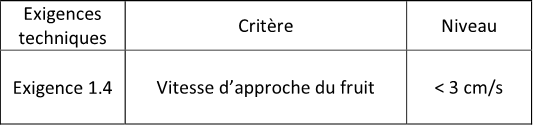
\includegraphics[width=.9\textwidth]{png/fig1}
\end{center}
\end{minipage}\hfill
\begin{minipage}[c]{.47\linewidth}
\begin{center}
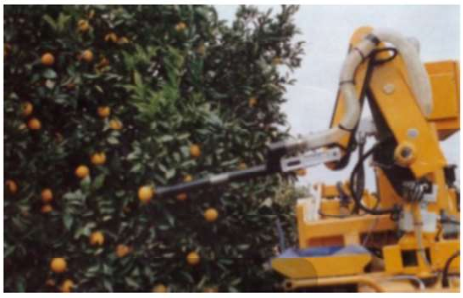
\includegraphics[width=.9\textwidth]{png/fig2}
\end{center}
\end{minipage}

\begin{center}
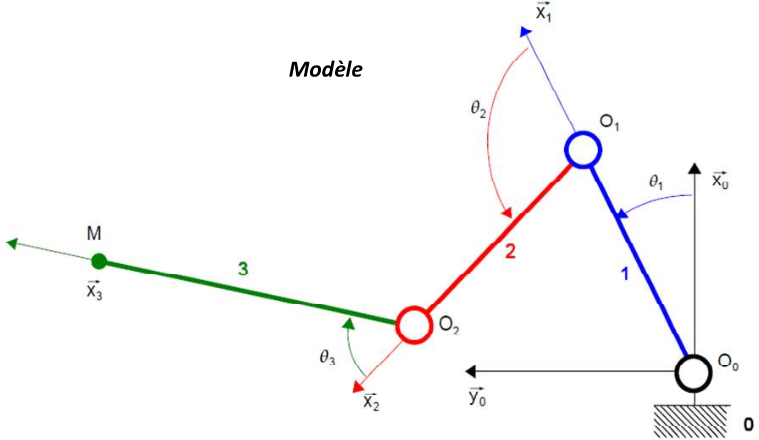
\includegraphics[width=.5\textwidth]{png/fig3}
\end{center}

\subparagraph{}
\textit{Construire les figures planes de repérage/paramétrage puis exprimer les vecteurs vitesse instantanée de rotation $\vecto{1}{0}$, $\vecto{2}{1}$, $\vecto{3}{2}$.} 
\ifthenelse{\boolean{prof}}{
\begin{corrige}

\couleursfigureplane{black}{blue}
\figureplanerep{x_0}{x_1}{y_0}{y_1}{z_0}{\theta_1}{0}{1}{3}
\couleursfigureplane{blue}{red}
\figureplanerep{x_1}{x_2}{y_1}{y_2}{z_0}{\theta_2}{1}{2}{3}
\couleursfigureplane{red}{green}
\figureplanerep{x_2}{x_3}{y_2}{y_3}{z_0}{\theta_3}{2}{3}{3}
$$
\vecrot{1}{0}=\dot\theta_1\vz{0} \quad \quad
\vecrot{2}{1}=\dot\theta_2\vz{0} \quad \quad
\vecrot{3}{2}=\dot\theta_3\vz{0}
$$
\end{corrige}}{}

\subparagraph{}
\textit{Déterminer $\vectv{O_1}{1}{0}$.}
\ifthenelse{\boolean{prof}}{
\begin{corrige}
\begin{align*}
\vecvit{O_1}{1}{0}&=\vecvit{O_0}{1}{0}+\vecrot{1}{0}\wedge\gv{O_0 O_1}\\
	&=\dot\theta_1\vz{0}\wedge R\vx{1}\\
\vecvit{O_1}{1}{0}&=R\dot\theta_1\vy{1}
\end{align*}
\end{corrige}}{}


\subparagraph{}
\textit{Déterminer $\vectv{O_2}{2}{0}$.}
\ifthenelse{\boolean{prof}}{
\begin{corrige}
\begin{align*}
\vecvit{O_2}{2}{0}&=\vecvit{O_1}{2}{0}+\vecrot{2}{0}\wedge\gv{O_1 O_2}\\
	&=\vecvit{O_1}{2}{1}+\vecvit{O_1}{1}{0}+(\vecrot{2}{1}+\vecrot{1}{0})\wedge\gv{O_1 O_2}\\
	&=R\dot\theta_1\vy{1}+(\dot\theta_2+\dot\theta_1)\vz0\wedge R\vx2\\
\vecvit{O_2}{2}{0}=R\dot\theta_1\vy{1}+R(\dot\theta_2+\dot\theta_1)\vy{2}
\end{align*}

\end{corrige}}{}

\subparagraph{}
\textit{Déterminer $\vectv{M}{3}{0}$.}
\ifthenelse{\boolean{prof}}{
\begin{corrige}
\begin{align*}
\vecvit{M}{3}{0}&=\vecvit{O_2}{3}{0}+\vecrot{3}{0}\wedge \gv{O_2 M}\\
	&=\vecvit{O_2}{3}{2}+\vecvit{O_2}{2}{0}+(\vecrot{3}{2}+\vecrot{2}{1}+\vecrot{1}{0})\wedge \gv{O_2 M}\\
	&=R\dot\theta_1\vy{1}+R(\dot\theta_2+\dot\theta_1)\vy{2}+(\dot\theta_3+\dot\theta_2+\dot\theta_1)\vz{0}\wedge L\vx{3}\\
\vecvit{M}{3}{0}&=R\dot\theta_1\vy{1}+R(\dot\theta_2+\dot\theta_1)\vy{2} +L(\dot\theta_3+\dot\theta_2+\dot\theta_1)\vy{3}
\end{align*}

\end{corrige}}{}

\subparagraph{}
\textit{Dans la configuration de rapprochement horizontal, ($\theta_2=\pi-2\theta_1$ et $\theta_3=\theta_1-\dfrac{\pi}{2}$) montrer que $\vectv{M}{3}{0}\cdot \vect{x_0}=0$et déterminer $||\vectv{M}{3}{0}||$.}
\ifthenelse{\boolean{prof}}{
\begin{corrige}

\systeq{
\theta_2&=\pi-2\theta_1\\
\theta_3&=\theta_1-\dfrac{\pi}{2}
}

\systeq{
\dot\theta_2&=-2\dot\theta_1\\
\dot\theta_3&=\theta_1
}
\begin{align*}
\vecvit{M}{3}{0}& =R\dot\theta_1\vy{1} +R(\dot\theta_2+\dot\theta_1)\vy{2} +L(\dot\theta_3+\dot\theta_2+\dot\theta_1)\vy{3}\\
	&=R\dot\theta_1\vy{1}-R\dot\theta_1\vy{2}+L(\dot\theta_1-2\dot\theta_1+\dot\theta_1)\vy{3}\\
	&=R\dot\theta_1(\vy{1}-\vy{2})
\intertext{Or}
\vy{1}&=\cos\theta_1\vy{0}-\sin\theta_1\vx{0}\\
\vy{2}&=\cos(\underbrace{\theta_1+\theta_2}_{\pi-\theta_1})\vy{0}- \sin(\underbrace{\theta_1+\theta_2}_{\pi-\theta_1})\vx0\\
	&=-\cos\theta_1\vy{0}-\sin\theta_1\vx{0}
\intertext{D'où}
\vy1-\vy2&=2\cos\theta_1\vy0\\
\intertext{Ainsi}
\vecvit{M}{3}{0}=2R\dot\theta_1\cos\theta_1\vy0
\end{align*}

Ce qui prouve que $\vecvit{M}{3}{0}\cdot\vx{0}=0$ et que :
$$
\left|\left|\vecvit{M}{3}{0}\right|\right|=2R\dot\theta_1\cos\theta_1
$$

\end{corrige}}{}


\subparagraph{}
\textit{Déterminer la valeur numérique de la vitesse maximale (R = 48 cm, L = 72 cm et $\dot{\theta_1}= 0,08 tr/min$ ) et conclure quant à la capacité du robot à satisfaire le critère de vitesse d'approche du fruit du cahier des charges. }
\ifthenelse{\boolean{prof}}{
\begin{corrige}
Application numérique : 
\systeq{
R&=0.48\ m\\
L&=0.72\ m\\
\dot\theta_1 &=0,08\text{ tr/min}\\
	&=0,00838\text{ rad/s}
}

La valeur maximale de $\left|\left|\vecvit{M}{3}{0}\right|\right|$ est atteinte pour $\theta_1=0$, ce qui donne :
\begin{align*}
\left|\left|\vecvit{M}{3}{0}\right|\right|&=2R\dot\theta_1\\
	&=0,00804\text{ m/s}\\
	&=0,8\text{ cm/s}
\end{align*}

\fbox{Le cahier des charges est bien respecté, car $\left|\left|\vecvit{M}{3}{0}\right|\right|<3\text{ cm/s}$}

\end{corrige}}{}

\section*{Manège Magic Arms } 
\setcounter{subparagraph}{0}

La manège Magic Arms dont la modélisation ainsi qu'un extrait de cahier des charges fonctionnel est composé d'une structure métallique d'environ $12\; m$ de haut avec deux bras mobiles. Les passagers s'assoient sur 39 pièces disposées sur une plate-forme tournante. Dès que tous les passagers sont assis et attachés, la nacelle tourne autour de son axe, le bras principal (bras 1) et le bras secondaires (bras 2), liés l'un à l'autre au début du cycle, commencent à tourner. Après 9 secondes, le maximum de hauteur est atteint et les deux bras se désindexent et se mettent à tourner indépendamment l'un de l'autre. Tous les mouvements sont pilotés par ordinateur. 

\begin{center}
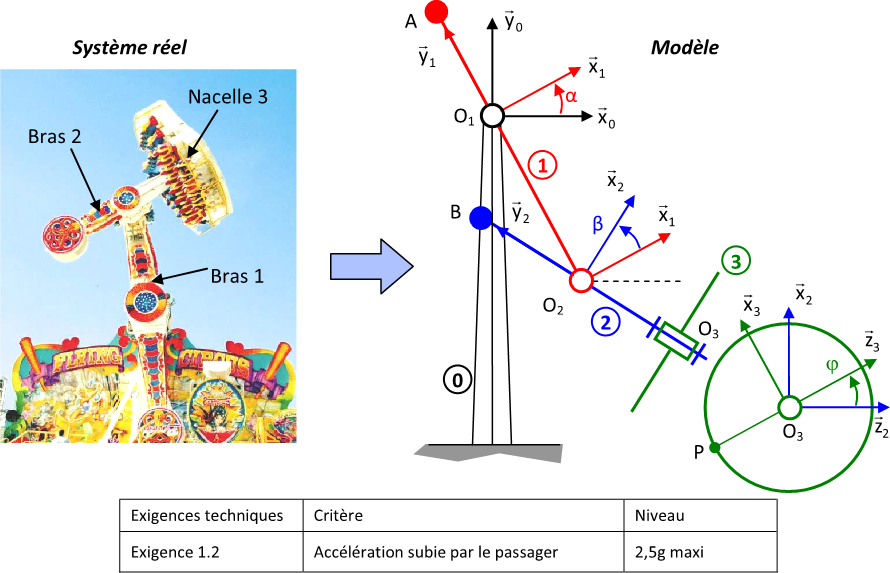
\includegraphics[width=.9\textwidth]{png/img1}
\end{center}

Le manège, schématisé ci-dessus, comporte :
\begin{itemize}
\item un bras principal 1 assimilé à une barre $AO_1O_2$. Il est en liaison pivot parfait d'axe $(O_1,\vect{z_1})$ caractérisée par le paramètre $\alpha$ avec le bâti 0. On pose $\vect{O_1O_2}=-l_1\vect{y_1}$;
\item un bras secondaire 2 assimilé à une barre $BO_2O_3$. Il est en liaison pivot parfait d'axe $(O_2,\vect{z_2})$ caractérisée par le paramètre $\beta$ avec le bras principal 1. On pose $\vect{O_2O_3}=-l_2\vect{y_2}$;
\item une nacelle 3 assimilée à un disque de centre $O_3$ et de rayon $R$. Elle est en liaison parfaite d'axe $(O_3,\vect{y_2})$ caractérisée par le paramètre $\varphi$ avec le bras 2. On s'intéresse plus particulièrement à un passager considéré comme un point matériel $P$ tel que $\vect{O_3P}=-R\vect{z_3}$.
\end{itemize}
\subparagraph{}
\textit{Construire les figures planes associées au schéma cinématique.}
\ifthenelse{\boolean{prof}}{
\begin{corrige}
\couleursfigureplane{black}{red}
\figureplanerep{x_0}{x_1}{y_0}{y_1}{z_0}{\alpha}{0}{1}{3}
\couleursfigureplane{red}{blue}
\figureplanerep{x_1}{x_2}{y_1}{y_2}{z_0}{\beta}{1}{2}{3}
\couleursfigureplane{blue}{green}
\figureplanerep{z_0}{z_3}{x_2}{x_3}{y_2}{\varphi}{2}{3}{3}

\end{corrige}}{}

\subparagraph{}
\textit{Calculer $\vecto{1}{0}$, $\vecto{2}{1}$ et $\vecto{3}{2}$.}
\ifthenelse{\boolean{prof}}{
\begin{corrige}
\begin{align*}
\vecrot{1}{0}&=\dot\alpha\vz0\\
\vecrot{2}{1}&=\dot\beta\vz0\\
\vecrot{3}{2}&=\dot\varphi\vy2\\
\end{align*}
\end{corrige}}{}

\vspace{.3cm}

On admet que $\vecto{3}{0}=\vecto{3}{2}+\vecto{2}{1}+\vecto{1}{0}$.

\subparagraph{}
\textit{Calculer $\vecto{2}{0}$ et $\vecto{3}{0}$.}
\ifthenelse{\boolean{prof}}{
\begin{corrige}
\begin{align*}
\vecrot{2}{0}&=\vecrot{2}{1}+\vecrot{1}{0}\\
	&=(\dot\alpha+\dot\beta)\vz0\\
\vecrot{3}{0}&=\vecrot{3}{2}+\vecrot{2}{0}\\
	&=(\dot\alpha+\dot\beta)\vz0+\dot\varphi\vy2
\end{align*}

\end{corrige}}{}

\subparagraph{}
\textit{Calculer les produits vectoriels suivants : $\vect{z_2}\wedge\vect{z_3}$,
$\vect{x_3}\wedge\vect{x_2}$, $\vect{x_3}\wedge\vect{z_2}$,
$\vect{z_2}\wedge\vect{z_1}$, $\vect{x_2}\wedge\vect{x_0}$,
$\vect{x_3}\wedge\vect{z_0}$.}
\ifthenelse{\boolean{prof}}{
\begin{corrige}

\begin{align*}
\vz2 \wedge \vz3 &=\sin\varphi \vy2\\
\vx3 \wedge\vx2 &= -\sin\varphi \vy2\\
\vx3 \wedge \vz2&= -\sin\left(\dfrac{\pi}{2}+\varphi\right)\vy2\\
	&=-\cos\varphi\vy2\\
\vz2 \wedge \vz1 &= \vec{0}\\
\vx2 \wedge \vx0 &= \left(\cos\beta\vx1+\sin\beta\vy1\right)\wedge\vx0\\
	&=-\cos\beta\sin\alpha\vz0 - \sin\beta\sin\left(\dfrac{\pi}{2}+\alpha\right)\vz0\\
	&=(-\cos\beta\sin\alpha-\sin\beta\cos\alpha)\vz0\\
	&=-\sin(\beta+\alpha)\vz0\\
\vx3\wedge\vz0 &= -\sin\left(\dfrac{\pi}{2}+\varphi\right)\vy2\\
	&=-\cos\varphi\vy2
\end{align*}

\end{corrige}}{}


\subparagraph{}
\textit{Calculer $\vectv{O_2}{2}{0}$, $\vectv{O_3}{3}{0}$ et $\vectv{P}{3}{0}$.}
\ifthenelse{\boolean{prof}}{
\begin{corrige}
\begin{align*}
\vecvit{O_2}{2}{0}&={\vecvit{O_2}{2}{1}}+\vecvit{O_2}{1}{0}\\
	&={\vecvit{O_1}{1}{0}}+\vecrot{1}{0}\wedge\gv{O_1 O_2}\\
	&= \dot\alpha\vz0 \wedge (-l_1 \vy1) \\
{\vecvit{O_2}{2}{0}}{= l_1\dot\alpha\vx1}\\
\vecvit{O_3}{3}{0}&={\vecvit{O_3}{3}{2}}+\vecvit{O_3}{2}{0}\\
	&=\vecvit{O_2}{2}{0}+\vecrot{2}{0}\wedge \gv{O_2 O_3}\\
	&=l_1\dot\alpha\vx1+(\dot\alpha+\dot\beta)\vz0\wedge (-l_2 \vy2)\\
{\vecvit{O_3}{3}{0}}{=l_1\dot\alpha\vx1+l_2(\dot\alpha+\dot\beta)\vx2}\\
\vecvit{P}{3}{0}&=\vecvit{O_3}{3}{0}+\vecrot{3}{0}\wedge\gv{O_3 P}\\	&=l_1\dot\alpha\vx1+l_2(\dot\alpha+\dot\beta)\vx2+ \left((\dot\alpha+\dot\beta)\vz0+\dot\varphi\vy2\right)\wedge(-R\vz3)\\
{\vecvit{P}{3}{0}}{=l_1\dot\alpha\vx1+l_2(\dot\alpha+\dot\beta)\vx2-R\sin\varphi(\dot\alpha+\dot\beta)\vy2-R\dot\varphi\vx3}
\end{align*}
\end{corrige}}{}

\vspace{.3cm}

On donne l'évolution des vitesses angulaires des moteurs du manège en fonction du temps.
\begin{center}
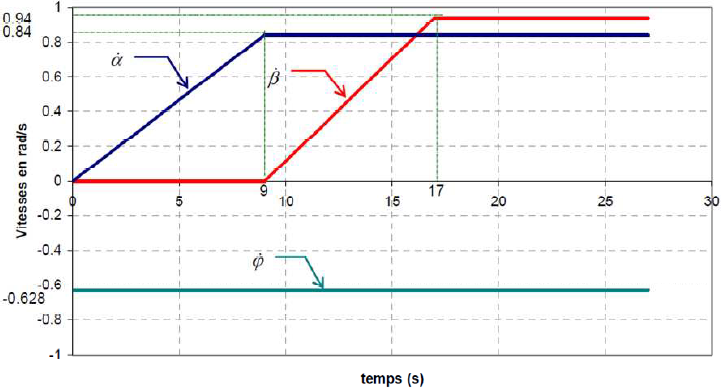
\includegraphics[width=.9\textwidth]{png/img2}
\end{center}

\subparagraph{\label{lab}}
\textit{Déterminer les valeurs des paramètres $\dot{\alpha}$, $\dot{\beta}$ et $\dot{\varphi}$
puis l'expression analytique des positions angulaires $\alpha(t)$ et $\beta(t)$ et $\varphi(t)$ dans l'intervalle de temps $[17;27]$ secondes en sachant qu'à l'instant $t=17\;s$, on a $\alpha=10,5\; rad$, $\beta=3,76\; rad$ et $\varphi=-10,676\; rad$.}
\ifthenelse{\boolean{prof}}{
\begin{corrige}

Dans l'intervalle de temps compris entre 17 et 27 secondes, les vitesses angulaires sont constantes.

$$
\systeq{
{\dot\alpha}{=0,84\text{ rad/s}}\\
{\dot\beta}{=0,94\text{ rad/s}}\\
{\dot\varphi}{=-0,628\text{ rad/s}}
}
$$

Ainsi, par intégration :
\begin{align*}
\alpha (t)-\alpha(17)&=\int_{17}^t \dot\alpha d\tau \\
%\alpha (t)-10,5&=0,84(t-17) \\
%{\alpha (t) }{= 0,84(t-17) + 10,5}\\	
%\beta (t)-\beta(17)&=\int_{17}^t \dot\beta d\tau \\
%\beta (t)-3,76&=0,94(t-17) \\
%{\beta (t) }{= 0,94(t-17) + 3,76}	\\
%\varphi (t)-\varphi(17)&=\int_{17}^t \dot\varphi d\tau \\
%\varphi (t)+10,676&=-0,628(t-17) \\
%{\varphi (t) }{= -0,628(t-17) -10,676}	\\
\end{align*}
\end{corrige}}{}

\subparagraph{}
\textit{Déterminer les valeurs numériques à l'instant $t_1=19,8\; s$ de $\alpha$, $\beta$ et $\varphi$.}
\ifthenelse{\boolean{prof}}{
\begin{corrige}

Pour $t=19,8$ s,
\[
\systeq{
\alpha&=0,84 \times (19,8-17) + 10,5=\boxed{12,85\text{ rad}}\\
\beta&=0,94\times (19,8-17) +3,76 = \boxed{6,39\text{ rad}}\\
\varphi &= -0,628\times (19,8-17) -10,676 =\boxed{12,43\text{ rad}}
}
\]

\end{corrige}}{}

\subparagraph{}
\textit{On pose $\vectv{P}{3}{0}=V_{x2}\vect{x_2}+V_{y2}\vect{y_2}+V_{z2}\vect{z_2}$. Déterminer les expressions littérales de $V_{x2}$, $V_{x2}$, $V_{z2}$ puis les valeurs numériques de à $t_1=19,8\;s.$} (On donne : $l_1=3,9\;m$, $l_2=2,87\;m$, $R=2,61\;m$.)
\ifthenelse{\boolean{prof}}{
\begin{corrige}

Il s'agit de projeter le vecteur \vecvit{P}{3}{0} dans la base $(\vx2, \vy2 ,\vz0)$. En effet, le vecteur \vz2 est identique au vecteur \vz0.
\begin{align*}
\vecvit{P}{3}{0}&=V_{x2}\vx2 +V_{y2}\vy2 + V_{z2}\vz0\\
V_{x2}&=\vecvit{P}{3}{0}\cdot\vx2\\
	&=\left(l_1\dot\alpha\vx1+l_2(\dot\alpha+\dot\beta)\vx2-R\sin\varphi(\dot\alpha+\dot\beta)\vy2-R\dot\varphi\vx3\right)\cdot\vx2\\
{V_{x2}}{=l_1 \dot\alpha\cos\beta+l_2 (\dot\alpha+\dot\beta) -R \dot\varphi\cos\varphi}\\
V_{y2}&=\vecvit{P}{3}{0}\cdot\vy2\\
	&=\left(l_1\dot\alpha\vx1+l_2(\dot\alpha+\dot\beta)\vx2-R\sin\varphi(\dot\alpha+\dot\beta)\vy2-R\dot\varphi\vx3\right)\cdot\vy2\\
{V_{y2}}{=-l_1\dot\alpha\sin\beta-R\sin\varphi(\dot\alpha+\dot\beta)}\\
V_{z2}&=\vecvit{P}{3}{0}\cdot\vy2\\
	&=\left(l_1\dot\alpha\vx1+l_2(\dot\alpha+\dot\beta)\vx2-R\sin\varphi(\dot\alpha+\dot\beta)\vy2-R\dot\varphi\vx3\right)\cdot\vz0\\
{V_{z2}}{=R\dot\varphi\sin\varphi}
\end{align*}

Valeurs numériques à $t=19,8$ s :

\begin{align*}
V_{x2}&=3,9\times 0,84 \times \cos (6,39) + 2,87  \times (0,84 + 0,94) + 2,61 \times 0,628 \times \cos (12,43) \\
	&=\boxed{9,99\text{ m/s}}\\
V_{y2}&=-3,9 \times 0,84 \times \sin(6,39) - 2,61 \times \sin(12,43) \times (0,84 + 0,94)\\
	&=\boxed{-0,28\text{ m/s}}\\
V_{z2}&=-2,61\times 0,628 \times \sin(12,43) \\
	&=\boxed{-0,22 \text{ m/s}}
\end{align*}

\end{corrige}}{}

\subparagraph{}
\textit{Calculer $\vect{\Gamma\left(P\in3/0 \right)}$.}
\ifthenelse{\boolean{prof}}{
\begin{corrige}

\begin{align*}
\vecacc{P}{3}{0}&=\gderivect{\vecvit{P}{3}{0}}{0}\\
	&=\dfrac{\dd}{\dd t}\left( l_1\dot\alpha\vx1+l_2(\dot\alpha+\dot\beta)\vx2-R\sin\varphi(\dot\alpha+\dot\beta)\vy2-R\dot\varphi\vx3 \right)_0 \\
	&=l_1 \ddot\alpha\vx1+l_1 \dot\alpha\underbrace{\derivect{\vx1}{0}}_{\dot\alpha\vy1} + l_2(\ddot\alpha + \ddot\beta)\vx2+ l_2(\dot\alpha+\dot\beta)\underbrace{\derivect{\vx2}{0}}_{(\dot\alpha+\dot\beta)\vy2}-R\dot\varphi\cos\varphi(\dot\alpha+\dot\beta)\vy2\\
	&\phantom{==}-R\sin\varphi(\ddot\alpha+\ddot\beta)\vy2-R\sin\varphi(\dot\alpha+\dot\beta)\underbrace{\derivect{\vy2}{0}}_{-(\dot\alpha+\dot\beta)\vx2}-R\ddot\varphi\vx3 -R\dot\varphi\derivect{\vx3}{0}\\
\derivect{\vx3}{0}&={\derivect{\vx3}{3}}+\vecrot{3}{0}\wedge\vx3\\
		&=\left((\dot\alpha+\dot\beta)\vz0+\dot\varphi\vy2\right)\wedge\vx3\\
		&=(\dot\alpha+\dot\beta)\cos\varphi\vy2-\dot\varphi\vz3
		\end{align*}
		
D'où :
\begin{align*}
\vecacc{P}{3}{0}&=l_1 \ddot\alpha\vx1+l_1 \dot\alpha^2\vy1 + l_2(\ddot\alpha + \ddot\beta)\vx2+ l_2(\dot\alpha+\dot\beta)^2\vy2-2R\dot\varphi\cos\varphi(\dot\alpha+\dot\beta)\vy2\\
	& -R\sin\varphi(\ddot\alpha+\ddot\beta)\vy2+R\sin\varphi(\dot\alpha+\dot\beta)^2\vx2-R\ddot\varphi\vx3 +R\dot\varphi^2\vz3
\end{align*}


\end{corrige}}{}

\subparagraph{}
\textit{Calculer $\vect{\Gamma\left(P\in3/0 \right)}$ dans l'intervalle de temps $[17;27]$ secondes pour lequel les vitesses angulaires sont constantes.}
\ifthenelse{\boolean{prof}}{
\begin{corrige}

Dans le cas ou les vitesses angulaires sont constantes, les accélérations angulaires $\ddot\alpha$, $\ddot\beta$, et $\ddot\varphi$ sont nulles. L'expression de \vecacc{P}{3}{0} se simplifie donc :
\begin{align*}
{\vecacc{P}{3}{0}}{=l_1 \dot\alpha^2\vy1 + l_2(\dot\alpha+\dot\beta)^2\vy2-2R\dot\varphi\cos\varphi(\dot\alpha+\dot\beta)\vy2+ R\sin\varphi(\dot\alpha+\dot\beta)^2\vx2 +R\dot\varphi^2\vz3}\\
\end{align*}

\end{corrige}}{}

\vspace{.3cm}

Le graphe ci-dessous, obtenu par simulation numérique, présente le module de la vitesse du passager $P$ par rapport au bâti 0 ainsi que le module de l'accélération du passager $P$ par rapport au bâti 0 en fonction du temps. 
\begin{center}
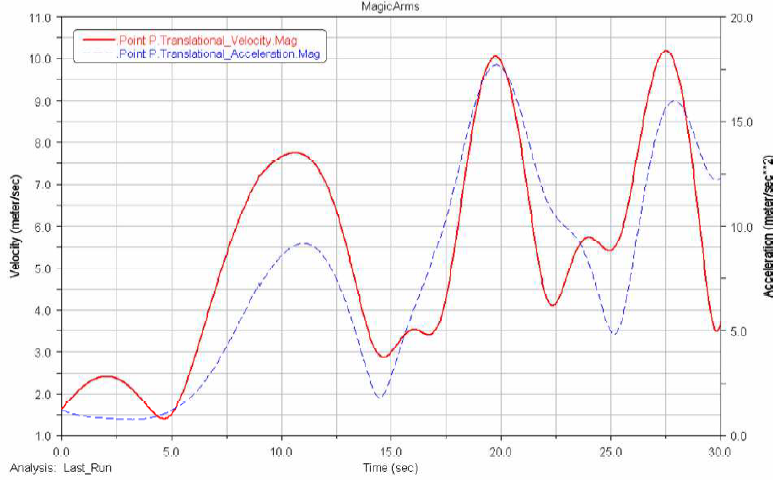
\includegraphics[width=.9\textwidth]{png/img3}
\end{center}

\subparagraph{}
\textit{Comparer les résultats obtenus à la question \ref{lab} à ceux du graphe pour le temps $t_1=19,8\;s.$.}
\ifthenelse{\boolean{prof}}{
\begin{corrige}

Le graphe montre qu'à $t=19,8$ s, l'intensité du vecteur \vecvit{P}{3}{0} vaut 10 m/s. Or  d'après la question~8, 
\begin{align*}
\left|\left|\vecvit{P}{3}{0}\right|\right|&=\sqrt{V_{x2}^2+V_{y2}^2+V_{z2}^2}\\
	&=\sqrt{9,99^2+0,28^2+0,22^2}\\
	&=\boxed{10\text{ m/s} }
\end{align*}

On constate que le calcul littéral nous donne le même résultat que l'exploitation de la courbe.

\end{corrige}}{}

\subparagraph{}
\textit{Relever l'accélération maximale subie par le passager et conclure vis-à-vis du CdCF.}
\ifthenelse{\boolean{prof}}{
\begin{corrige}
D'après la courbe de l'accélération (en pointillés), la valeur maximale de l'accélération subie par le passager vaut 17,5 m/s\up{2}. Le cahier des charges exige que l'accélération maximale ne dépasse pas 2,5 $g$, soit 24,5 m/s\up{2}. Le cahier des charges est donc respecté.

\end{corrige}}{}

\end{document}
